% This template can serve as a starting point for your BSc thesis. You are allowed to modify it as long as you adhere to the requirements from the Thesis Manual.
\documentclass[a4paper,11pt]{article}
\usepackage[T2A]{fontenc}
\usepackage[utf8]{inputenc}
\usepackage[main=bulgarian, english]{babel}
\usepackage{graphbox}
\usepackage{multirow}
\usepackage{xcolor}
\usepackage{listings}
\lstset{basicstyle=\ttfamily,
  showstringspaces=false,
  commentstyle=\color{red},
  keywordstyle=\color{blue}
}
\usepackage{float}
\usepackage{multirow}
\usepackage{tabularx}

% FILL OUT THE DETAILS BELOW:
\author{Даниел Халачев}
\title{MandelTest}
% \date{An optional custom date, the default is today}
\newcommand{\subtitle}{Скалируемост на теста на Манделброт с кеш адаптивност и \\ статично и динамично балансиране }
\newcommand{\studentnumber}{62547}
\newcommand{\program}{Софтуерно инеженерство}
\newcommand{\supervisor}{проф. д-р. Васил Цунижев}
\newcommand{\secondassesor}{ас. Христо Христов}
\renewcommand{\lstlistingname}{Програмен код}

\usepackage[onehalfspacing]{setspace} % Increase line spacing
\usepackage[margin=2.5cm]{geometry} % Modify margins
\usepackage{graphicx,booktabs,apacite} % Packages for images, tables, and APA citations

\begin{document}

\begin{titlepage}
\makeatletter
\begin{center}
	\textsc{Софийски университет "Св. Климент Охридски"}
	\par \textsc{Факултет по математика и информатика}
	\par Специалност "\program"

	\vfill \hrule height .08em \bigskip
	\par\huge\@title\bigskip
	\par\Large\subtitle\bigskip
	\hrule height .08em\normalsize
	
	\vfill
	\includegraphics[width=\textwidth,height=0.25\textheight,keepaspectratio]{SU.png} % The EUR logo, but this could also be another image
	\vfill
	
	\begin{tabular}{ll}
		\toprule
		Изготвил: & \@author\\
		Факултетен номер: & \studentnumber\\
		Дата: & \@date\\
		\bottomrule
	\end{tabular}
	
	\vfill
\end{center}
\makeatother
\end{titlepage}

\begin{abstract}
\begin{figure}[H]
    \centering
    \includegraphics[width=0.9\linewidth]{images/Mandelbrot.png}
    \caption{\centering Изображение на фрактала на Манделброт в областта \newline $Re\in\left[-2.50;1.30\right], Im\in\left[-1.1;1.1\right]$}
    \label{fig:mandelbrot}
\end{figure}    
\end{abstract}

\cleardoublepage
\tableofcontents
\cleardoublepage
\pagenumbering{arabic}

\section{Въведение}
Фракталите са структури, които са самоподобни със собствените си части. Те се създават чрез рекурсивни или итеративни процеси, изпълнени неограничен брой пъти. В резултат, фракталите не могат да бъдат изобразени в тяхната цялост, а единствено чрез техни приближения. 
Терминът \emph{фрактал} е въведен за първи път от Беноа Манделброт през 1975г., като думата произхожда от латинската \emph{fractus} - начупен, което отразява свойството, отличаващо фракталите от други структури - тяхното самоподобие, видимо по границите на структурите. Въпреки това, фракталите са известни на човечеството много по-рано - като форми, които се срещат в природата, или като графики на математически функции (функция на Вайерщрас, снежинка на Кох и др.). 
\subsection{Фрактал на Манделброт}
Един от най-популярните фрактали е този на Манделброт. Множеството на Манделброт е множеството от всички комплексни числа $c$, такива, че функцията $f_c(z)=z^2+c$ не е разходяща за $z=0$, тоест е ограничена. Казано по-просто, това са всички комплексни числа $c$, такива, че редицата $\left\{a_i\right\}^\infty=f_c(0), f_c(f_c(0)), ... = c, f_c(c), f_c(f_c(c)), ...$ е ограничена по абсолютна стойност. 
Например за $c_1=1$ редицата $\left\{a_i\right\}=0, 1, 2, 5, 26, ...$. Тя не е разходяща, тоест е неограничена, следователно числото $c_1=1$ не принадлежи на множеството на Манделброт. 
От друга страна, за $c_2=-1$, $\left\{a_i\right\}=-1, 0, -1, 0, -1, ...$ е ограничена, следователно числото $c_2=-1$ принадлежи на множеството на Манделброт. 
Понеже множеството на Манделброт е компактно, то се побира в кръг с радиус 2 и център - началото на координатната система. Затова, за да определим дали редицата $\left\{a_i\right\}^\infty=f_c(0), f_c(f_c(0)), ... = c, f_c(c), f_c(f_c(c)), ...$ е ограничена по абсолютна стойност, е достатъчно да проверим дали $\left\|a_i\right\|\leq 2$. 
\subsection{Последователен алгоритъм за изобразяване на множеството на Манделброт}
Фракталът за първи път е дефиниран и нарисуван от Робърт Брукс и Питър Мателски през 1978г., но Беноа Манделброт първи го визуализира на компютър - през 1980г., и затова фракталът е наречен в негова чест. 
Генерирането на изображението на компютър се основава на математическата дефиниция. По дължината на изображението се нанасят реалните части, а по височината на изображението - имагинерните части на комплексните числа $c$. Определя се праг, или максимален брой итерации (членове на редицата), според които да определим дали редицата е ограничена. Дефинира се палитра от цветове, които кодират колко бързо редицата се доближава до ограничението. Цветовете са толкова на брой, колкото са и членовете на редицата, която проверяваме. Колкото по-голям е максималният брой итерации, толкова по-богата е палитрата и толкова по-детайлно е изображението. 
По-конкретно, за максимален брой итерации 1024, за всеки пиксел от изображението:
\begin{enumerate}
    \item изчисляваме стойността на $c$ в дадения пиксел
    \item изчисляваме $a_0, a_1,\dots, a_{1024}$, като спираме изчислението, ако $\left\|a_i\right\|\leq 2$. 
    \item ако сме стигнали до $a_{1024}$ и $\left\|a_{1024}\right\|\leq 2$, то оцветяваме пиксела в черно, което означава, че точката принадлежи на множеството на Манделброт. Ако сме спрели изчислението по-рано, оцветяваме точката толкова тъмно, колкото по-рано е спряло изчислението. 
\end{enumerate}
\section{Анализ}
\subsection{Техники за паралелен алгоритъм на теста на Манделброт}
\subsubsection{Смущаващо паралелни алгоритми [1]}
Смущаващо паралелни алгоритми са такива алгоритми, при които се изискват минимални усилия за разделянето на изчислителния проблем на паралелни процеси. Такива проблеми се отличават с ограничена или никаква комуникация между отделните процеси. Генерирането на Множеството на Манделброт е подходящ пример за такива процеси, защото няма зависимост по данни - всеки пиксел се изчислява независимо от всеки друг, а освен това липсва необходимост от комуникация между отделните нишки, т.е. алгоритъмът е асинхронен.

Максимална ефективност се постига, когато всички процесорни ядра са заети за възможно най-дълго време. 
Но един от процесите трябва да раздели проблема и да „раздаде“ задачите. Такива архитектури се наричат \emph{Master-Slave}. 

\begin{figure}[H]
    \centering
    \includegraphics[width=0.9\linewidth]{images/embarassingly_parallel1.png}
    \caption{Архитектура на смущаващо паралелна програма}
    \label{fig:emb-parallel-1}
\end{figure}
Комбинацията от SPMD и Master Slave носи предимствата и на двата модела - позволява разпределение на задачите, но минимална комуникация между процесите и ефективна работа и на „главната“ нишка.
\begin{figure}[H]
    \centering
    \includegraphics[width=0.9\linewidth]{images/embarassingly_parallel2.png.png}
    \caption{Архитектура на смущаващо паралелна SPMD + Master-Slave програма}
    \label{fig:emb-parallel-2}
\end{figure}
\subsubsection{Ефективно генериране на множеството на Манделброт [2]}
Статията разглежда ефективното генериране на множеството на Манделброт от гледна точка на приложението му в криптирането. Първо се доказва, че изчислителният проблем може да се паралелизира чрез правилата на Bernstein. Разглеждат се три подхода за балансиране при \emph{Master-Slave} архитектура:
\begin{enumerate}
    \item \textbf{Делене на блокове} - изображението се разделя на блокове от равен брой последователни редове. Ако броят нишки е $p$, то изображението се поделя на $p$ блока. 
    \item \textbf{Динамично балансиране на принципа \emph{First Come, First Served}} - изображението се поделя на части, или задачи. Всяка задача се състои от един ред. Задава се по една задача на всяка нишка. След като дадена нишка приключи изчислението си, получава нова от главната нишка до изчерпването на всички задачи. 
    \item \textbf{Статично циклично балансиране} - изображението отново се поделя на редове. Предварително се определя коя нишка кои редове ще получи. 
\end{enumerate}
Резултатите при генерирането на изображение с размери $8000\times8000$ с $2000$ итерации са следните:
\begin{table}[H]
    \centering
    \begin{tabular}{|c|c|c|c|c|}
    \hline
        \textbf{N} & \textbf{Теоретична} & \textbf{\multirow{2}{*}{Статично блоково}} & \textbf{Динамично} & \textbf{\multirow{2}{*}{Статично циклично}} \\
        & \textbf{скорост} & \textbf{балансиране} & \textbf{балансиране} & \textbf{балансиране} \\ \hline
        2 & 1.999440 & 1.97812 & 1.00396 & 1.99000 \\ \hline
        4 & 3.96659 & 2.05984 & 2.98414 & 3.96060 \\ \hline
        8 & 7.84583 & 2.49809 & 6.77486 & 7.60671 \\ \hline
        16 & 15.35350 & 3.97305 & 13.33375 & 13.37449 \\ \hline
        32 & 29.43820 & 7.37966 & 23.72932 & 22.87749 \\ \hline
        $\infty$ & 356.22764 & - & - & - \\ \hline
    \end{tabular}
    \caption{Постигнато ускорение в статията Effective Mandelbrot Computation}
\end{table}

\begin{figure}[H]
    \centering
    \includegraphics[width=0.9\linewidth]{images/Efficient Generation of Mandelbrot Set.png}
    \caption{Ускорение в статията Efficient Generation of Mandelbrot Set}
    \label{fig:efficient-generation}
\end{figure}
\begin{enumerate}
    \item \textbf{Делене на блокове} - при паралелизъм $p=2$ резултатите са близки до теоретичния лимит и останалите два подхода. Това не е изненадващо, защото изображението се поделя на две части, които са симетрични. При нарастване на паралелизма се проявява недостатъкът на подхода и постигнатото ускорение е значително по-малко. Причината е, че блоковете вече не са симетрични и работата на нишките не е балансирана справедливо. 
    \item \textbf{Динамично балансиране} - при паралелизъм $p=2$ не се постига почти никакво ускорение. Причината е, че главната нишка просто предава задачата на единствената второстепенна нишка. Колкото повече нараства паралелизма, толкова по-справедлива е подялбата на работата. При 32 нишки ускорението става категорично по-добро от това при статично циклично балансиране. Причината - комуникационният свръхтовар се компенсира от по-ефективното използване на процесорното време. 
    \item \textbf{Статично циклично балансиране} - подходът запазва консистентно добро ускорение при всички стойности на паралелизма, защото се осигурява ефективно балансиране при минимизиран свръхтовар. 
\end{enumerate} 
\subsubsection{Паралелно генериране на множеството на Манделброт [3]}
Статията \emph{Parallel generation of a Mandelbrot set} разглежда две схеми на паралелизация на алгоритъма:
\begin{itemize}
    \item \textbf{Статично балансиране} - изображението се поделя на толкова области, колкото са и паралелните процеси. Главният процес също изчислява една област. 
    \item \textbf{Динамично балансиране} - главният процес има единствено управляваща роля. Изображението се поделя на задачи, които се раздават на процесите, докато не се изчерпят.
\end{itemize}
Тестването на ускорението включва няколко различни сценария:
\begin{enumerate}
    \item Изображение $12800\times12800$, поделено на области, които са правоъгълници. Видима е огромната разлика в постигнатото ускорение между статично и динамично балансиране. В допълнение се наблюдава силно проявена немотонна аномалия. И двете прояви не са изненадващи с оглед на неподходящата схема на балансиране. Множеството на Манделброт е компактно, следователно няколко области ще останат напълно празни, а други ще съдържат само точки от множеството. Именно затова схемата с динамично балансиране постига по-добро ускорение.
    \begin{figure}[H]
        \centering
        \includegraphics[width=0.9\linewidth]{images/mirco1.png}
        \caption{Ускорение при разделяне по области в статията \emph{Parallel generation of a Mandelbrot set}}
        \label{fig:enter-label}
    \end{figure}
    \item Изображение $1600\times1600$, поделено на редове или на колони. При схемата със статично балансиране се получава голямо разминаване между постигнатото ускорение по редове и по-колони, което е значително по-ниско. С оглед на еднаквата ширина и височина на изображението, възможно обяснение за явлението е избраната област за изобразяване на множеството, която не е упомената. Отново се появява немотононна аномалия, която би могла да бъде обяснена с възможен недостатък в паралелната имплементация на алгоритъма. Това предположение изглежда по-вероятно с оглед на постигнатия паралелизъм и в двата случая, който е значително по-нисък от теоретичния лимит според закона на Амдал. 
    \begin{figure}[H]
        \centering
        \includegraphics[width=0.9\linewidth]{images/mirco2.png}
        \caption{Статично циклично балансиране по редове и по колони в статията \emph{Parallel generation of a Mandelbrot set}}
        \label{fig:mirco-2}
    \end{figure}    
    Разликата между редове и колони по отношение на сложността на изчисление не оказва влияние върху имплементацията с динамично балансиране, което обяснява голямото сходство в полученото ускорение по редове и по колони. В допълнение, ускорението в този сценарий е много по-близко до теоретичния лимит, което говори за по-ефикасен алгоритъм. 
    \begin{figure}[H]
        \centering
        \includegraphics[width=0.9\linewidth]{images/mirco3.png}
        \caption{Динамично централизирано балансиране по редове и по колони в статията \emph{Parallel generation of a Mandelbrot set}}
        \label{fig:mirco-3}
    \end{figure}
\end{enumerate}
\subsubsection{Сравнение между MPI и OpenMP при генериране на множеството на Манделброт [4] }
Статията прави сравнение между \emph{Message Passing Interface} и \emph{Open Multi-Processing} технологиите за паралелно програмиране. \emph{OpenMP} технологията е изградена на принципа \emph{shared memory}, при което се постига паралелизъм на ниво нишки - задачите се изпълняват на нишки, част от \emph{един} процес. За разлика от \emph{OpenMP}, \emph{MPI} задачите се изпълняват от няколко процеса, които се съгласуват чрез предаване на съобщения. 
Тестването е проведено за различен брой итерации и паралелизъм, като са използвани две имплементации на \emph{MPI} и три схеми за балансиране за \emph{OpenMP} - статично, динамично и \emph{guided} (задачите не са с еднакъв размер - започва се с големи, но към края размерът им намалява с цел максимално точно балансиране):
\begin{figure}[H]
    \centering
    \includegraphics[width=0.9\linewidth]{images/mpi-vs-openmp.png}
    \caption{Постигнато ускорение в статията \emph{MPI} vs \emph{OpenMP}}
    \label{fig:mpi-vs-openmp}
\end{figure}
Всички варианти с \emph{message passing} изостават в сравнение с \emph{OpenMP} поради породения свръхтовар от обмена на съобщения. \emph{Shared memory} вариантът със статично балансиране постига по-добро ускорение. Най-добро ускорение постигат динамичното и \emph{guided} балансирането. Това е очаквано с оглед на факта, че декомпозицията е по брой пиксели (матрицата е представена в кода като едномерен масив) и статичното балансиране не е циклично. 
\subsection{Технологичен анализ}
\begin{table}[H]
    \centering
    \begin{tabularx}{\linewidth}{|c|X|}
        \hline
        \multirow{2}{*}{№} & \multirow{2}{*}{Платформа} \\
        & \\
        \hline
        [2] & \textbf{Intel® Xeon® Gold Processor}\newline
        L1d cache 576 KiB\newline
        L1i cache 576 KiB\newline
        Level 2 Cache 18 MiB\newline
        Level 3 Cache 24.75 MiB\newline
        Threads 18/36, hyper-threading – turned off\\
        \hline
        [3] & клъстер от 13 Intel quadcore 64-битови x86\_64 процесора с 2GB RAM\\
        \hline
        [4] & \textbf{AMD Ryzen™ 5 2500U Quad-Core}\newline
        Level 1 Cache 384 KB\newline
        Level 2 Cache 2 MB\newline
        Level 3 Cache 4 MB\\
        \hline
    \end{tabularx}
    \caption{Използвани платформи в различните източници}
    \label{tab:platforms}
\end{table}
\subsection{Сравнителна таблица}
\begin{table}[H]
    \centering
    \begin{tabularx}{\linewidth}{|c|X|X|X|X|X|c|}
        \hline
        \multirow{2}{*}{№} & \multirow{2}{*}{Балансиране} & \multirow{2}{*}{Размерност} & \multirow{2}{*}{Паралелизъм} & \multirow{2}{*}{Итерации} & \multirow{2}{*}{Грануларност} & \multirow{2}{*}{Ускорение} \\
        & & & & & & \\
        \hline
        [2] & Статично циклично по редове и по блокове от редове & $8000\times8000$ & $18/36$ & $2000$ & средна, фина & $11.9$ \\
        \hline
        [3] & Статично циклично по блокове, по редове и по колони; динамично централизирано & $1600\times1600$ $12800\times12800$ & $13/16$ & 1000 & едра, средна, фина & $6.5-7$ \\
        \hline
        [4] & Статично и динамично балансиране & $1024\times 1024$ & 4/8 & 100, 1000, 10000, 100000 & едра, средна, фина & $\sim3.25$\\
        \hline 
        MT & Статично циклично по редове; динамично централизирано & $3840\times2160$ & $16/32$ & $1024$ & едра, средна, фина & $12.483$\\
        \hline
    \end{tabularx}
    \caption{Сравнителна таблица}
    \label{tab:comparisson-table}
\end{table}

\section{Проектиране}
\subsection{Функционално проектиране}
Ще постигнем паралелизъм чрез декомпозиция по данни и асинхронен алгоритъм. Ще се стремим към архитектура от тип \emph{Single Program Multiple Data}, защото всеки процес ще изпълнява едни и същи като тип изчисления, но върху различни данни (различни пиксели). Архитектурата ще напомня и на \emph{Master-Slave}, защото първата нишка ще отговаря за разделянето на проблема между различните нишки и за тяхното стартиране. Комуникация ще се осъществява само при инициализирането на „второстепенните“ нишки и след завършването им, когато се определя цялото време за изчисление. Основният въпрос е как ще бъдат балансирани задачите между отделните процеси.
\subsubsection{Статично циклично балансиране}
Статичното циклично балансиране е подходящ подход за разпределението на задачите между отделните процеси. Изображението се поделя на ленти (по редове или по колони), като всеки процес получава за обработка (почти) равен брой несъседни ленти. Това позволява по-справедливо разпределение на работата, защото всеки процес ще получи области и с малка, и с голяма сложност на изчисление. 
\begin{figure}[H]
    \centering
    \includegraphics[width=0.9\linewidth]{images/Decomposition.png}
    \caption{Статично циклично балансиране при паралелизъм $p=4$}
    \label{fig:decomposition}
\end{figure}
\subsubsection{Динамично централизирано балансиране}
Друга възможна техника за балансиране на заданията е динамичното централизирано балансиране. Изображението се поделя на задания, които се съхраняват в опашка, като в началото всеки процес получава по едно задание. Процес, който свърши със заданието си, получава ново до изчерпването на всички задания в опашката. Този подход гарантира, че през повечето време процесите са заети, но налага интензивна комуникация между процесите. Този курсов проект ще извърши тестване и с динамично централизирано балансиране, освен със статично циклично, с цел анализ на свръхтовара. Очакването е породеният свръхтовар за този изчислителен проблем да направи решението с динамично централизирано балансиране по-бавно от имплементацията със статично циклично. 
\begin{figure}[H]
    \centering
    \includegraphics[width=0.9\linewidth]{images/threadpool.png}
    \caption{Динамично балансиране чрез опашка от задачи}
    \label{fig:threadpool}
\end{figure}
\subsubsection{Модел на системата}
Диаграмата на последователностите представя поредицата от стъпки в главния процес и една от всички $p-1$ стартирани нишки. Времето за обработка започва да се измерва непосредствено преди стартирането на нишките и приключва с края на работата на последната нишка. В него не се включва превръщането на таблицата от изчисления в изображения по предварително зададената палета, нито входно-изходни операции. 
\begin{figure}[H]
    \centering    \includegraphics[width=0.9\linewidth]{images/sequence.png}
    \caption{Диаграма на последователностите за главната и една произволна от второстепенните нишки}
    \label{fig:sequence}
\end{figure}
\subsection{Технологично проектиране}
\subsubsection{Тестова среда}
Тестването на имплементациите със статично циклично и динамично централизирано балансиране се осъществи на сървъра на адрес \emph{t5600.rmi.yaht.net}, който е със следните характеристики:
\begin{lstlisting}[]
[u62547@t5600 ~]$ lscpu
Architecture:        x86_64
CPU op-mode(s):      32-bit, 64-bit
Byte Order:          Little Endian
CPU(s):              32
On-line CPU(s) list: 0-31
Thread(s) per core:  2
Core(s) per socket:  8
Socket(s):           2
NUMA node(s):        2
Vendor ID:           GenuineIntel
CPU family:          6
Model:               45
Model name:          Intel(R) Xeon(R) CPU E5-2660 0 @ 2.20GHz
Stepping:            7
CPU MHz:             3000.000
CPU max MHz:         3000,0000
CPU min MHz:         1200,0000
BogoMIPS:            4389.39
Virtualization:      VT-x
L1d cache:           32K
L1i cache:           32K
L2 cache:            256K
L3 cache:            20480K
NUMA node0 CPU(s):   0-7,16-23
NUMA node1 CPU(s):   8-15,24-31
\end{lstlisting}
\subsubsection{Ръководство на потребителя}
Имплементацията със статично циклично балансиране се помещава в пакета \lstinline{src.balancing.constant}, с основен клас \lstinline{StaticMandelTest.java}. 
Имплементацията с динамично централизирано балансиране се помещава в пакета \lstinline{src.balancing.dynamic.pool}, с основен клас \lstinline{DynamicMandelTest.java}. 
За да се изпълни програмата, трябва първо да се компилират класовете ѝ, заедно с използваните библиотеки, например така:
\begin{lstlisting}[language=bash,caption={Компилиране на StaticMandelTest от директорията корен на проекта},breaklines=true]
javac -cp lib/commons-cli-1.5.0.jar:lib/commons-math3-3.6.1.jar src/balancing/constant/*
\end{lstlisting}
Когато се въвежда командата за изпълнение на компилираната програма, може да се променят настройките по подразбиране чрез следните командни параметри:
\begin{table}[H]
\centering
\begin{tabular}{|l|l|l|p{6cm}|}
\hline
\textbf{Опция} & \textbf{Пълна форма} & \textbf{Стойност по подразбиране} & \textbf{Упътване} \\
\hline
-w & --width & 3840px & Указва ширината на изображението в px \\
\hline
-h & --height & 2160px & Указва височината на изображението в px \\
\hline
-d & --dimensions & 2.50:1.30:1.1:1.1 & Указва крайните точки на изображението във формата $X_{min}:X_{max}:Y_{min}:Y_{max}$ \\
\hline
-p & --parallelism & 16 & Указва броя нишки за изпълнение на програмата \\
\hline
-o & --output & StaticMandel.png & Указва пътя до изображението, включително името на файла му. \\
% \hline
% -q & --quiet & false & Enables quiet mode, suppressing unnecessary output. \\
\hline
-i & --info & & Показва възможните опции на програмата \\
\hline
-c & --cols &  & Флаг без стойност. Ако се посочи, декомпозицията се прави по колони, а не по редове \\
\hline
-g & --granularity &  & Определя размера на задачите\\
\hline
\end{tabular}
\caption{Командни параметри на програмите \lstinline{StaticMandelTest} и \lstinline{DynamicMandelTest}}
\end{table}

Остава само програмата да се изпълни с желаните параметри, например по този начин:
\begin{lstlisting}[language=bash,caption={Изпълнение на програмата \lstinline{StaticMandelTest} с допълнително задаване на паралелизъм $p=4$}, breaklines=true, captionpos=b]
java -cp lib/commons-cli-1.5.0.jar:lib/commons-math3-3.6.1.jar:src balancing.constant.StaticMandelTest -p 4
\end{lstlisting}

Ако желаете да изпълните програмата многократно по тестовия план, можете да го направите чрез последователното изпълнение на скриптовете \lstinline{compileStaticMandel.sh} и \lstinline{runStaticMandel.sh} в директорията корен на проекта ето така:
\begin{lstlisting}[language=bash,caption={Компилиране и изпъление на програмата според тестовия план}, captionpos=b]
$ ./compileStaticMandel.sh
$ ./runStaticMandel.sh myCSV.csv
\end{lstlisting}
\textbf{Забележка: }Ръководството на потребителя е аналогично и за имплементацията с динамично централизирано балансиране. 
\subsubsection{Програмен език и системни извиквания}
\paragraph{}
Програмата е разработена на езика \lstinline{Java} и използва две външни библиотеки - \\ \lstinline{org.apache.commons.math3.6.1} - за класа \lstinline{Complex}, и \lstinline{org.apache.commons.cli-1.5.0} - за анализ на входните параметри. Библиотеките се предоставят заедно с програмните класове в папката \lstinline{libs} под формата на \lstinline{jar} файлове. \\
„Второстепенните“ нишки се създават чрез следния код:
\begin{lstlisting}[language=Java, caption={Инициализиране на $p-1$ нишки в Java}, captionpos=b]
workers = new Thread[NUMBER_OF_THREADS];
for (int workerIndex = 1; workerIndex < NUMBER_OF_THREADS; workerIndex++) {
    Runnable r = new StaticWorker(workerIndex);
    Thread t = new Thread(r);
    t.start();
    workers[workerIndex] = t;
}
\end{lstlisting}
Освен тях се задава работа и на "главната нишка" чрез \lstinline[language=Java]{new StaticWorker(0).run();}.
„Главната“ нишка „проверява“ дали останалите са свършили, като изпраща сигнал, след което заспива. Второстепенната нишка връща отговор, с което „събужда“ главната. Процесът се повтаря докато не постъпят сигнали от всички нишки, че са свършили изчисленията си. Това се осъществява чрез кода:
\begin{lstlisting}[language=Java, caption={Проверка на $p-1$ нишки в Java}, captionpos=b]
for (int j = 1; j < threads; ++j) {
    try {
        workers[j].join();
    } catch (Exception e) {
        e.printStackTrace();
    }
}
\end{lstlisting}
\section{Тестване}
В секциите по-долу са посочени резултатите от проведеното тестване, където $p$ е паралелизмът, $g$ - грануларността, $T_p^i$ - времето в милисекунди на $i$-тия опит при паралелизъм $p$, $T_p$ - най-малкото $T_p^i$, $S_p = \frac{T_1}{T_p}$ - ускорението, а $E=\frac{S_p}{p}$ - ефективността. 
\subsection{Статично циклично балансиране}
\begin{table}[H]
    \centering
    \begin{tabular}{|c|c|c|c|c|c|c|c|}
    \hline
        $p$ & $g$ & $T_p^1$ & $T_p^2$ & $T_p^3$ & $T_p=min\left\{T_p^{i}\right\}$ & $S_p = \frac{T_1}{T_p}$ & $E=\frac{S_p}{p}$\\ \hline
        1 & 1 & 29401 & 29403 & 29384 & 29384 & 1.000 & 1.000 \\ \hline
        2 & 1 & 15167 & 15153 & 15153 & 15153 & 1.939 & 0.970 \\ \hline
        4 & 1 & 13376 & 13468 & 13443 & 13376 & 2.197 & 0.549 \\ \hline
        8 & 1 & 8078 & 8071 & 8151 & 8071 & 3.641 & 0.455 \\ \hline
        12 & 1 & 5990 & 5889 & 5887 & 5887 & 4.991 & 0.416 \\ \hline
        16 & 1 & 4675 & 4671 & 4628 & 4628 & 6.349 & 0.397 \\ \hline
        24 & 1 & 3504 & 3386 & 3454 & 3386 & 8.678 & 0.362 \\ \hline
        32 & 1 & 3167 & 2953 & 2971 & 2953 & 9.951 & 0.311 \\ \hline
        1 & 4 & 29252 & 29263 & 29282 & 29252 & 1.005 & 1.005 \\ \hline
        2 & 4 & 15179 & 15189 & 15097 & 15097 & 1.946 & 0.973 \\ \hline
        4 & 4 & 8122 & 8091 & 8106 & 8091 & 3.632 & 0.908 \\ \hline
        8 & 4 & 4613 & 4620 & 4679 & 4613 & 6.370 & 0.796 \\ \hline
        12 & 4 & 3264 & 3373 & 3286 & 3264 & 9.002 & 0.750 \\ \hline
        16 & 4 & 2693 & 2778 & 2733 & 2693 & 10.911 & 0.682 \\ \hline
        24 & 4 & 2508 & 2517 & 2491 & 2491 & 11.796 & 0.492 \\ \hline
        32 & 4 & 2452 & 2464 & 2457 & 2452 & 11.984 & 0.374 \\ \hline
        1 & 16 & 29490 & 29378 & 29381 & 29378 & 1.000 & 1.000 \\ \hline
        2 & 16 & 15205 & 15056 & 14994 & 14994 & 1.960 & 0.980 \\ \hline
        4 & 16 & 7847 & 7846 & 7885 & 7846 & 3.745 & 0.936 \\ \hline
        8 & 16 & 4146 & 4194 & 4164 & 4146 & 7.087 & 0.886 \\ \hline
        12 & 16 & 3002 & 3002 & 2985 & 2985 & 9.844 & 0.820 \\ \hline
        16 & 16 & 2569 & 2508 & 2542 & 2508 & 11.716 & 0.732 \\ \hline
        24 & 16 & 2393 & 2400 & 2385 & 2385 & 12.320 & 0.513 \\ \hline
        32 & 16 & 2372 & 2354 & 2377 & 2354 & 12.483 & 0.390 \\ \hline
    \end{tabular}
    \caption{Тестов план при статично циклично балансиране}
\end{table}
\begin{figure}[H]
    \centering
    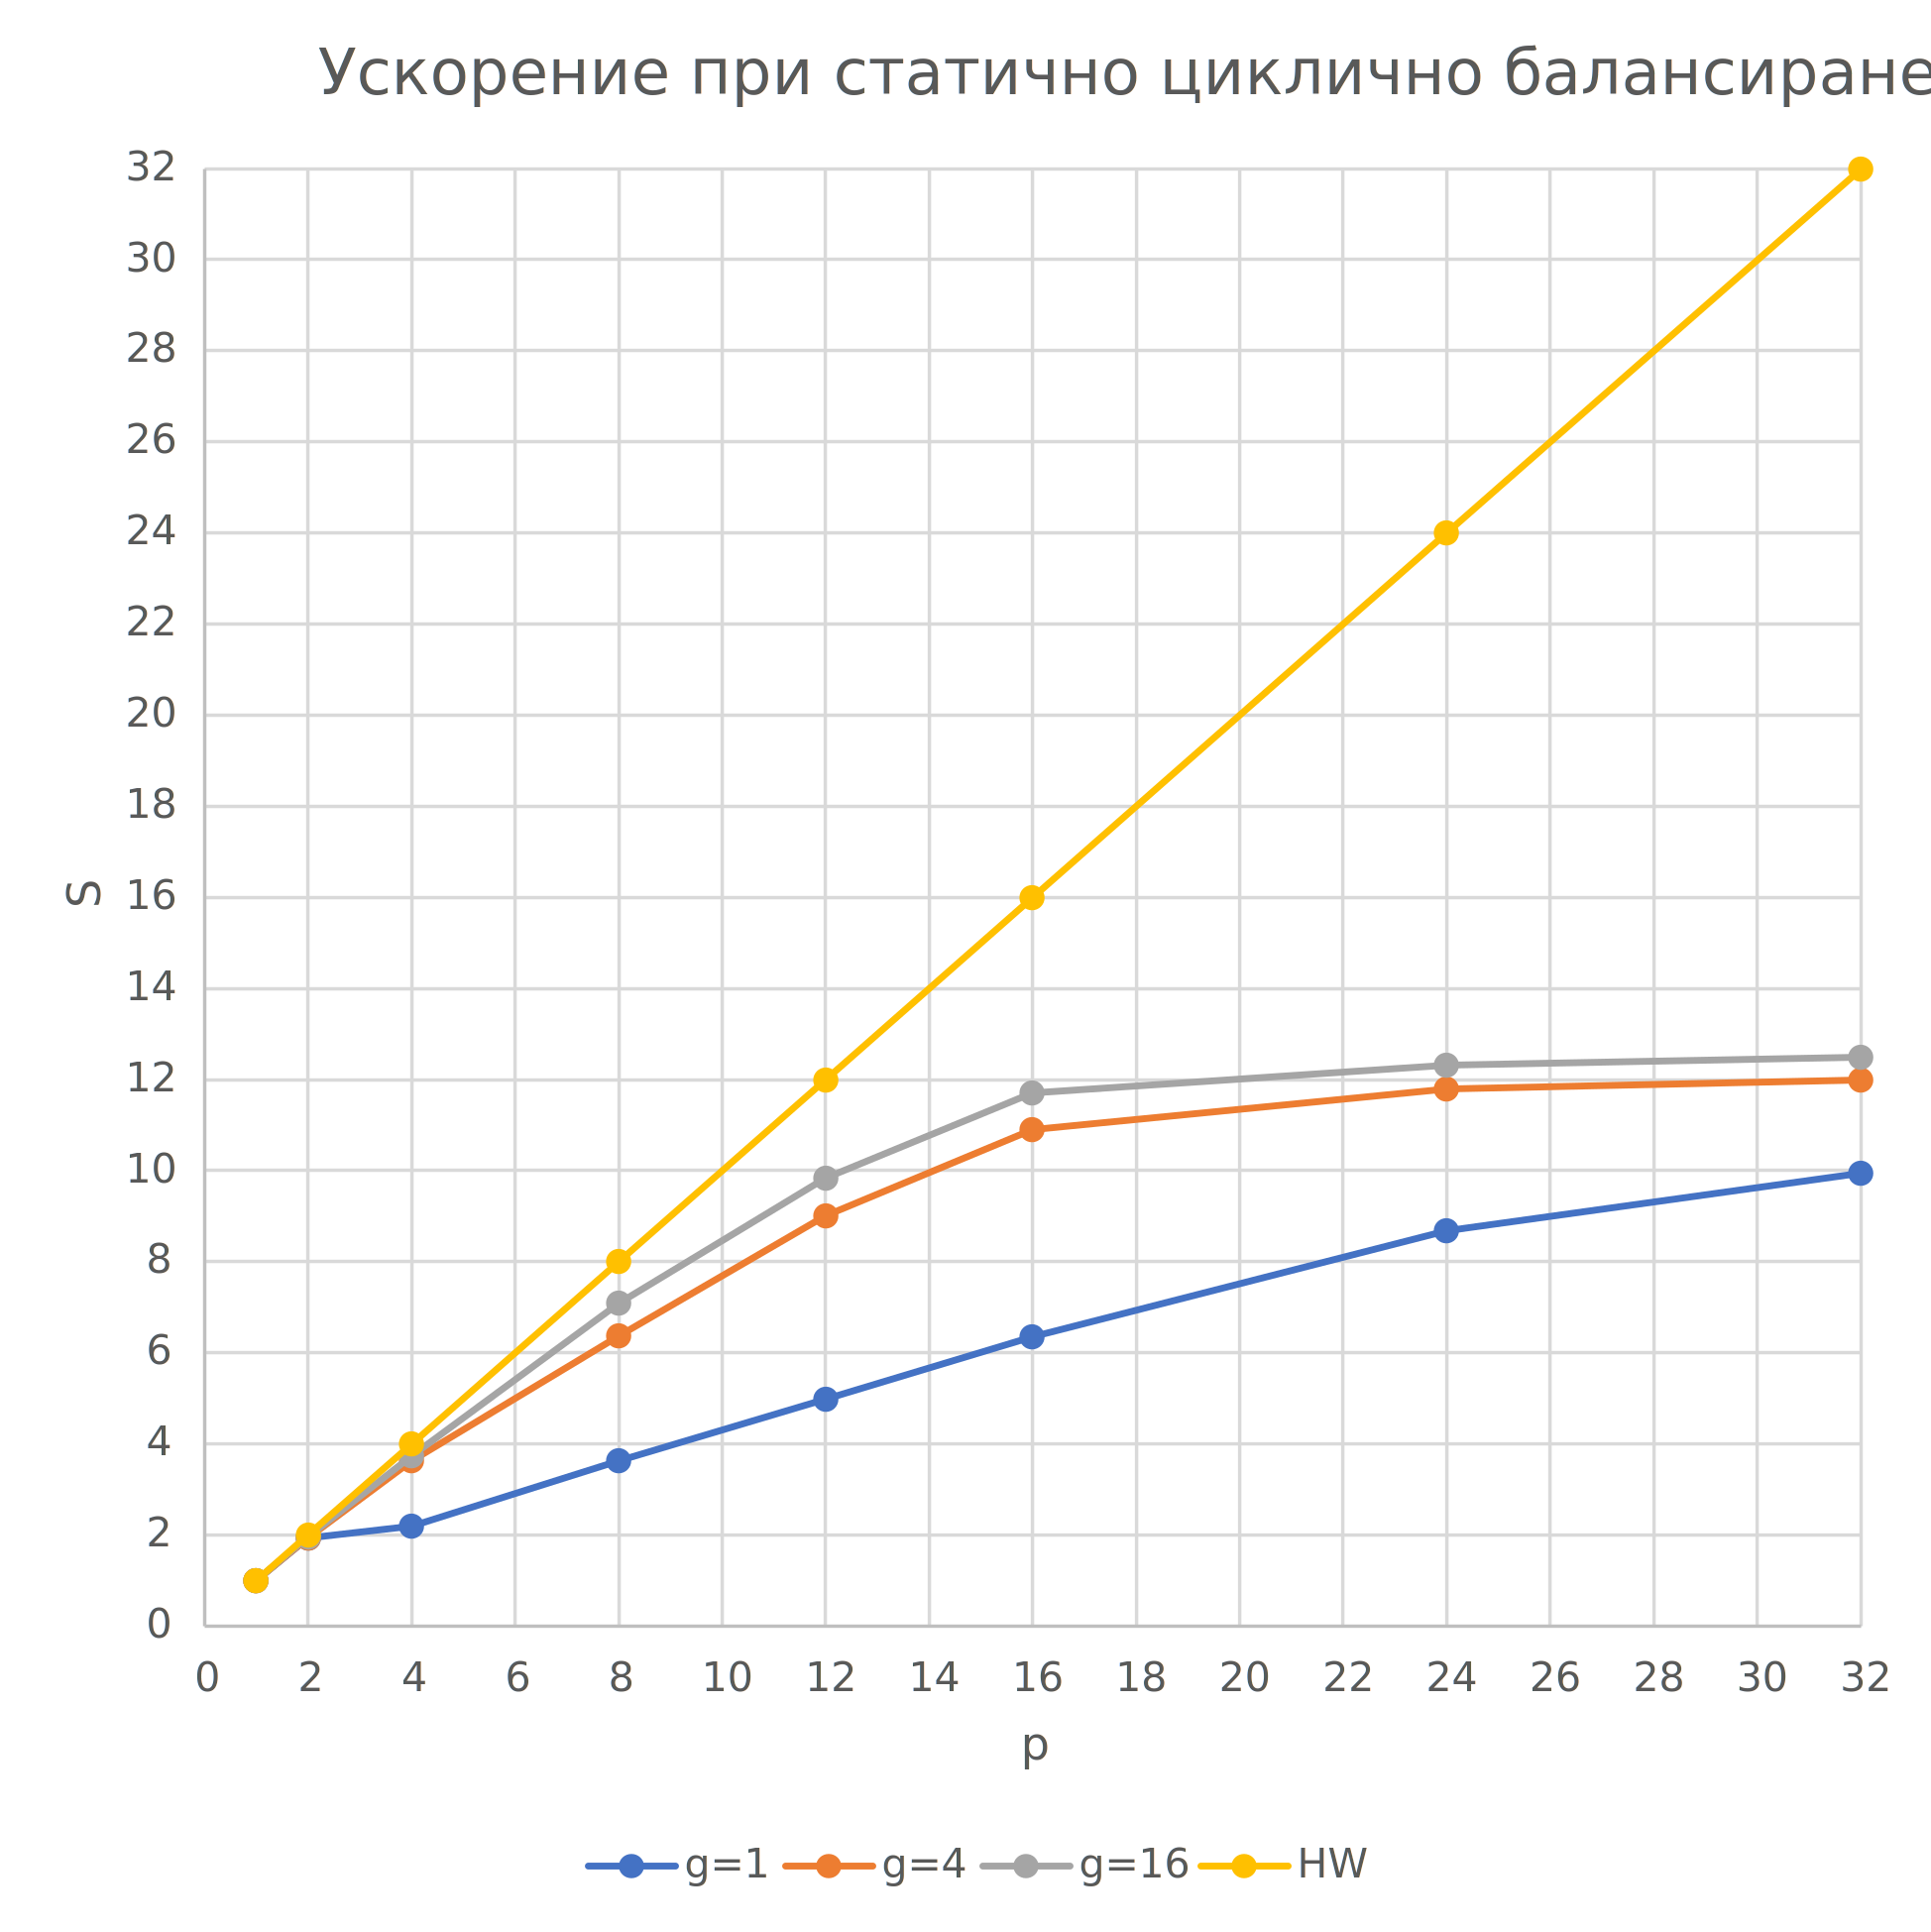
\includegraphics[width = 0.9\linewidth]{images/StaticMandelSpeedup.png}
    \caption{Ускорение при статично балансиране}
    \label{fig:static-speedup}
\end{figure}
\begin{figure}[H]
    \centering
    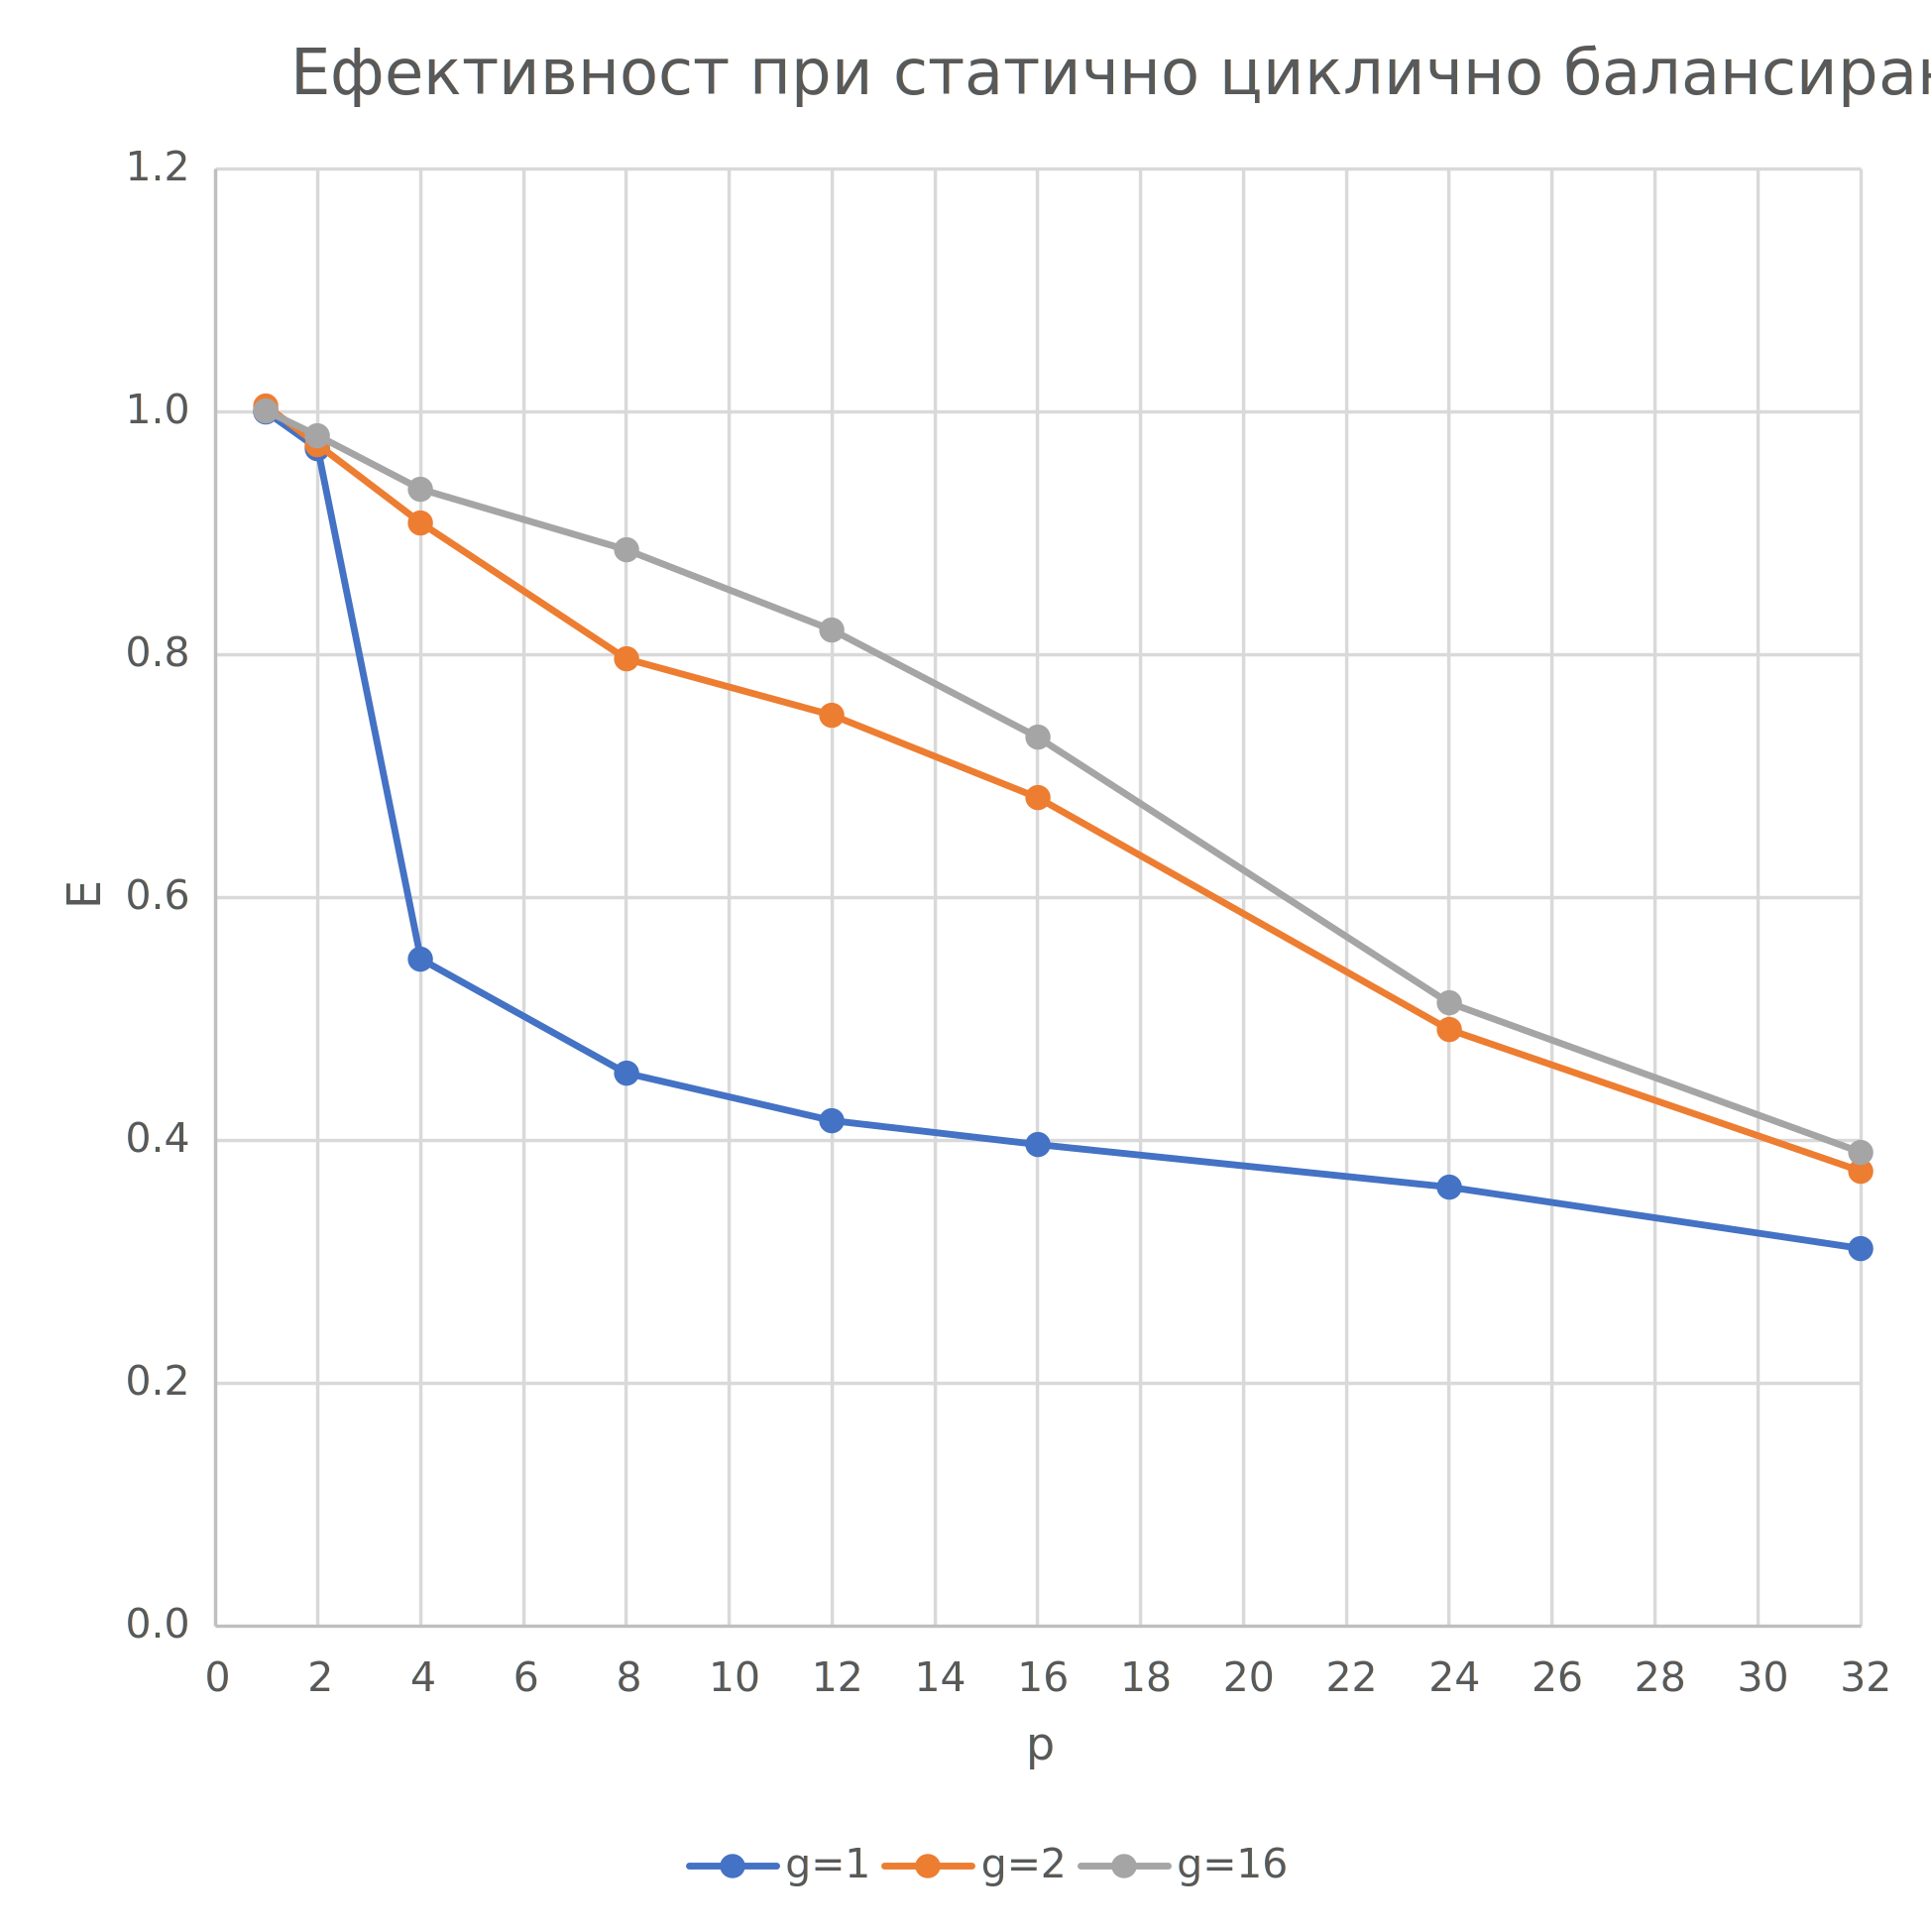
\includegraphics[width=0.9\linewidth]{images/StaticMandelEffectiveness.png}
    \caption{Ефективност при статично балансиране}
    \label{fig:static-effectiveness}
\end{figure}
От таблицата и графиките е видимо, че най-високото ускорение - $12.483$, е постигнато при грануларност $g=16$ и $32$ нишки. При тази грануларност е постигнат най-приспособен размер на данните спрямо L1D Cache. 
Особено видимо на графиката е минималното увеличение на ускорението при паралелизъм над $16$. Причината е, че сървърът разполага само с $16$ физически ядра, а $32$ са логическите ядра. Тоест, на всяко физическо ядро се падат по 2 нишки - това е т.нар. технология на \emph{Intel} - \emph{Hyperthreading}, която официално посочва очаквано подобрение до $30\%$. В случая, то е едва $2\%$. Ако игнорираме логическите ядра, постигнатият паралелизъм от $12.483$ при $p=16$ е сравнително близък до теоретичния лимит, посочен от закона на Амдал. 
В резултатите липсва немотонна аномалия, която е възможно да се прояви, ако алгоритъмът беше тестван при допълнителни стойности на паралелизъм - например $20, 28, 30$ и други. 
Наблюдават се минимални стойности на хиперлинейна аномалия за $p=1, g=4$, които могат да бъдат обяснени с неточно изчисление на времето на изпълнение на цялата програма, което все пак зависи от ядрото на операционната система. 
\subsection{Динамично централизирано балансиране}
\begin{table}[H]
    \centering
    \begin{tabular}{|c|c|c|c|c|c|c|c|}
    \hline
        $p$ & $g$ & $T_p^1$ & $T_p^2$ & $T_p^3$ & $T_p=min\left\{T_p^{i}\right\}$ & $S = \frac{T_1}{T_p}$ & $E=\frac{S_p}{p}$\\ \hline
        1 & 1 & 29430 & 29453 & 29525 & 29430 & 1.000 & 1.000 \\ \hline
        2 & 1 & 15236 & 15176 & 15319 & 15176 & 1.939 & 0.970 \\ \hline
        4 & 1 & 13311 & 13499 & 13325 & 13311 & 2.211 & 0.553 \\ \hline
        8 & 1 & 8491 & 8592 & 8593 & 8491 & 3.466 & 0.433 \\ \hline
        12 & 1 & 5959 & 6000 & 5957 & 5957 & 4.940 & 0.412 \\ \hline
        16 & 1 & 4660 & 4717 & 4839 & 4660 & 6.315 & 0.395 \\ \hline
        24 & 1 & 3450 & 3360 & 3374 & 3360 & 8.759 & 0.365 \\ \hline
        32 & 1 & 3350 & 3197 & 3073 & 3073 & 9.577 & 0.299 \\ \hline
        1 & 4 & 29460 & 29493 & 29460 & 29460 & 0.999 & 0.999 \\ \hline
        2 & 4 & 15164 & 15112 & 15169 & 15112 & 1.947 & 0.974 \\ \hline
        4 & 4 & 8141 & 8364 & 8182 & 8141 & 3.615 & 0.904 \\ \hline
        8 & 4 & 4707 & 4644 & 4578 & 4578 & 6.429 & 0.804 \\ \hline
        12 & 4 & 3311 & 3263 & 3334 & 3263 & 9.019 & 0.752 \\ \hline
        16 & 4 & 2673 & 2650 & 2779 & 2650 & 11.106 & 0.694 \\ \hline
        24 & 4 & 2497 & 2494 & 2500 & 2494 & 11.800 & 0.492 \\ \hline
        32 & 4 & 2470 & 2455 & 2518 & 2455 & 11.988 & 0.375 \\ \hline
        1 & 16 & 29347 & 29331 & 29480 & 29331 & 1.003 & 1.003 \\ \hline
        2 & 16 & 15136 & 15356 & 15090 & 15090 & 1.950 & 0.975 \\ \hline
        4 & 16 & 7810 & 7881 & 7749 & 7749 & 3.798 & 0.949 \\ \hline
        8 & 16 & 4179 & 4195 & 4191 & 4179 & 7.042 & 0.880 \\ \hline
        12 & 16 & 3054 & 3033 & 2992 & 2992 & 9.836 & 0.820 \\ \hline
        16 & 16 & 2490 & 2489 & 2471 & 2471 & 11.910 & 0.744 \\ \hline
        24 & 16 & 2453 & 2431 & 2428 & 2428 & 12.121 & 0.505 \\ \hline
        32 & 16 & 2375 & 2405 & 2359 & 2359 & 12.476 & 0.390 \\ \hline
    \end{tabular}
    \caption{Тестов план при динамично централизирано балансиране}
\end{table}
\begin{figure}[H]
    \centering
    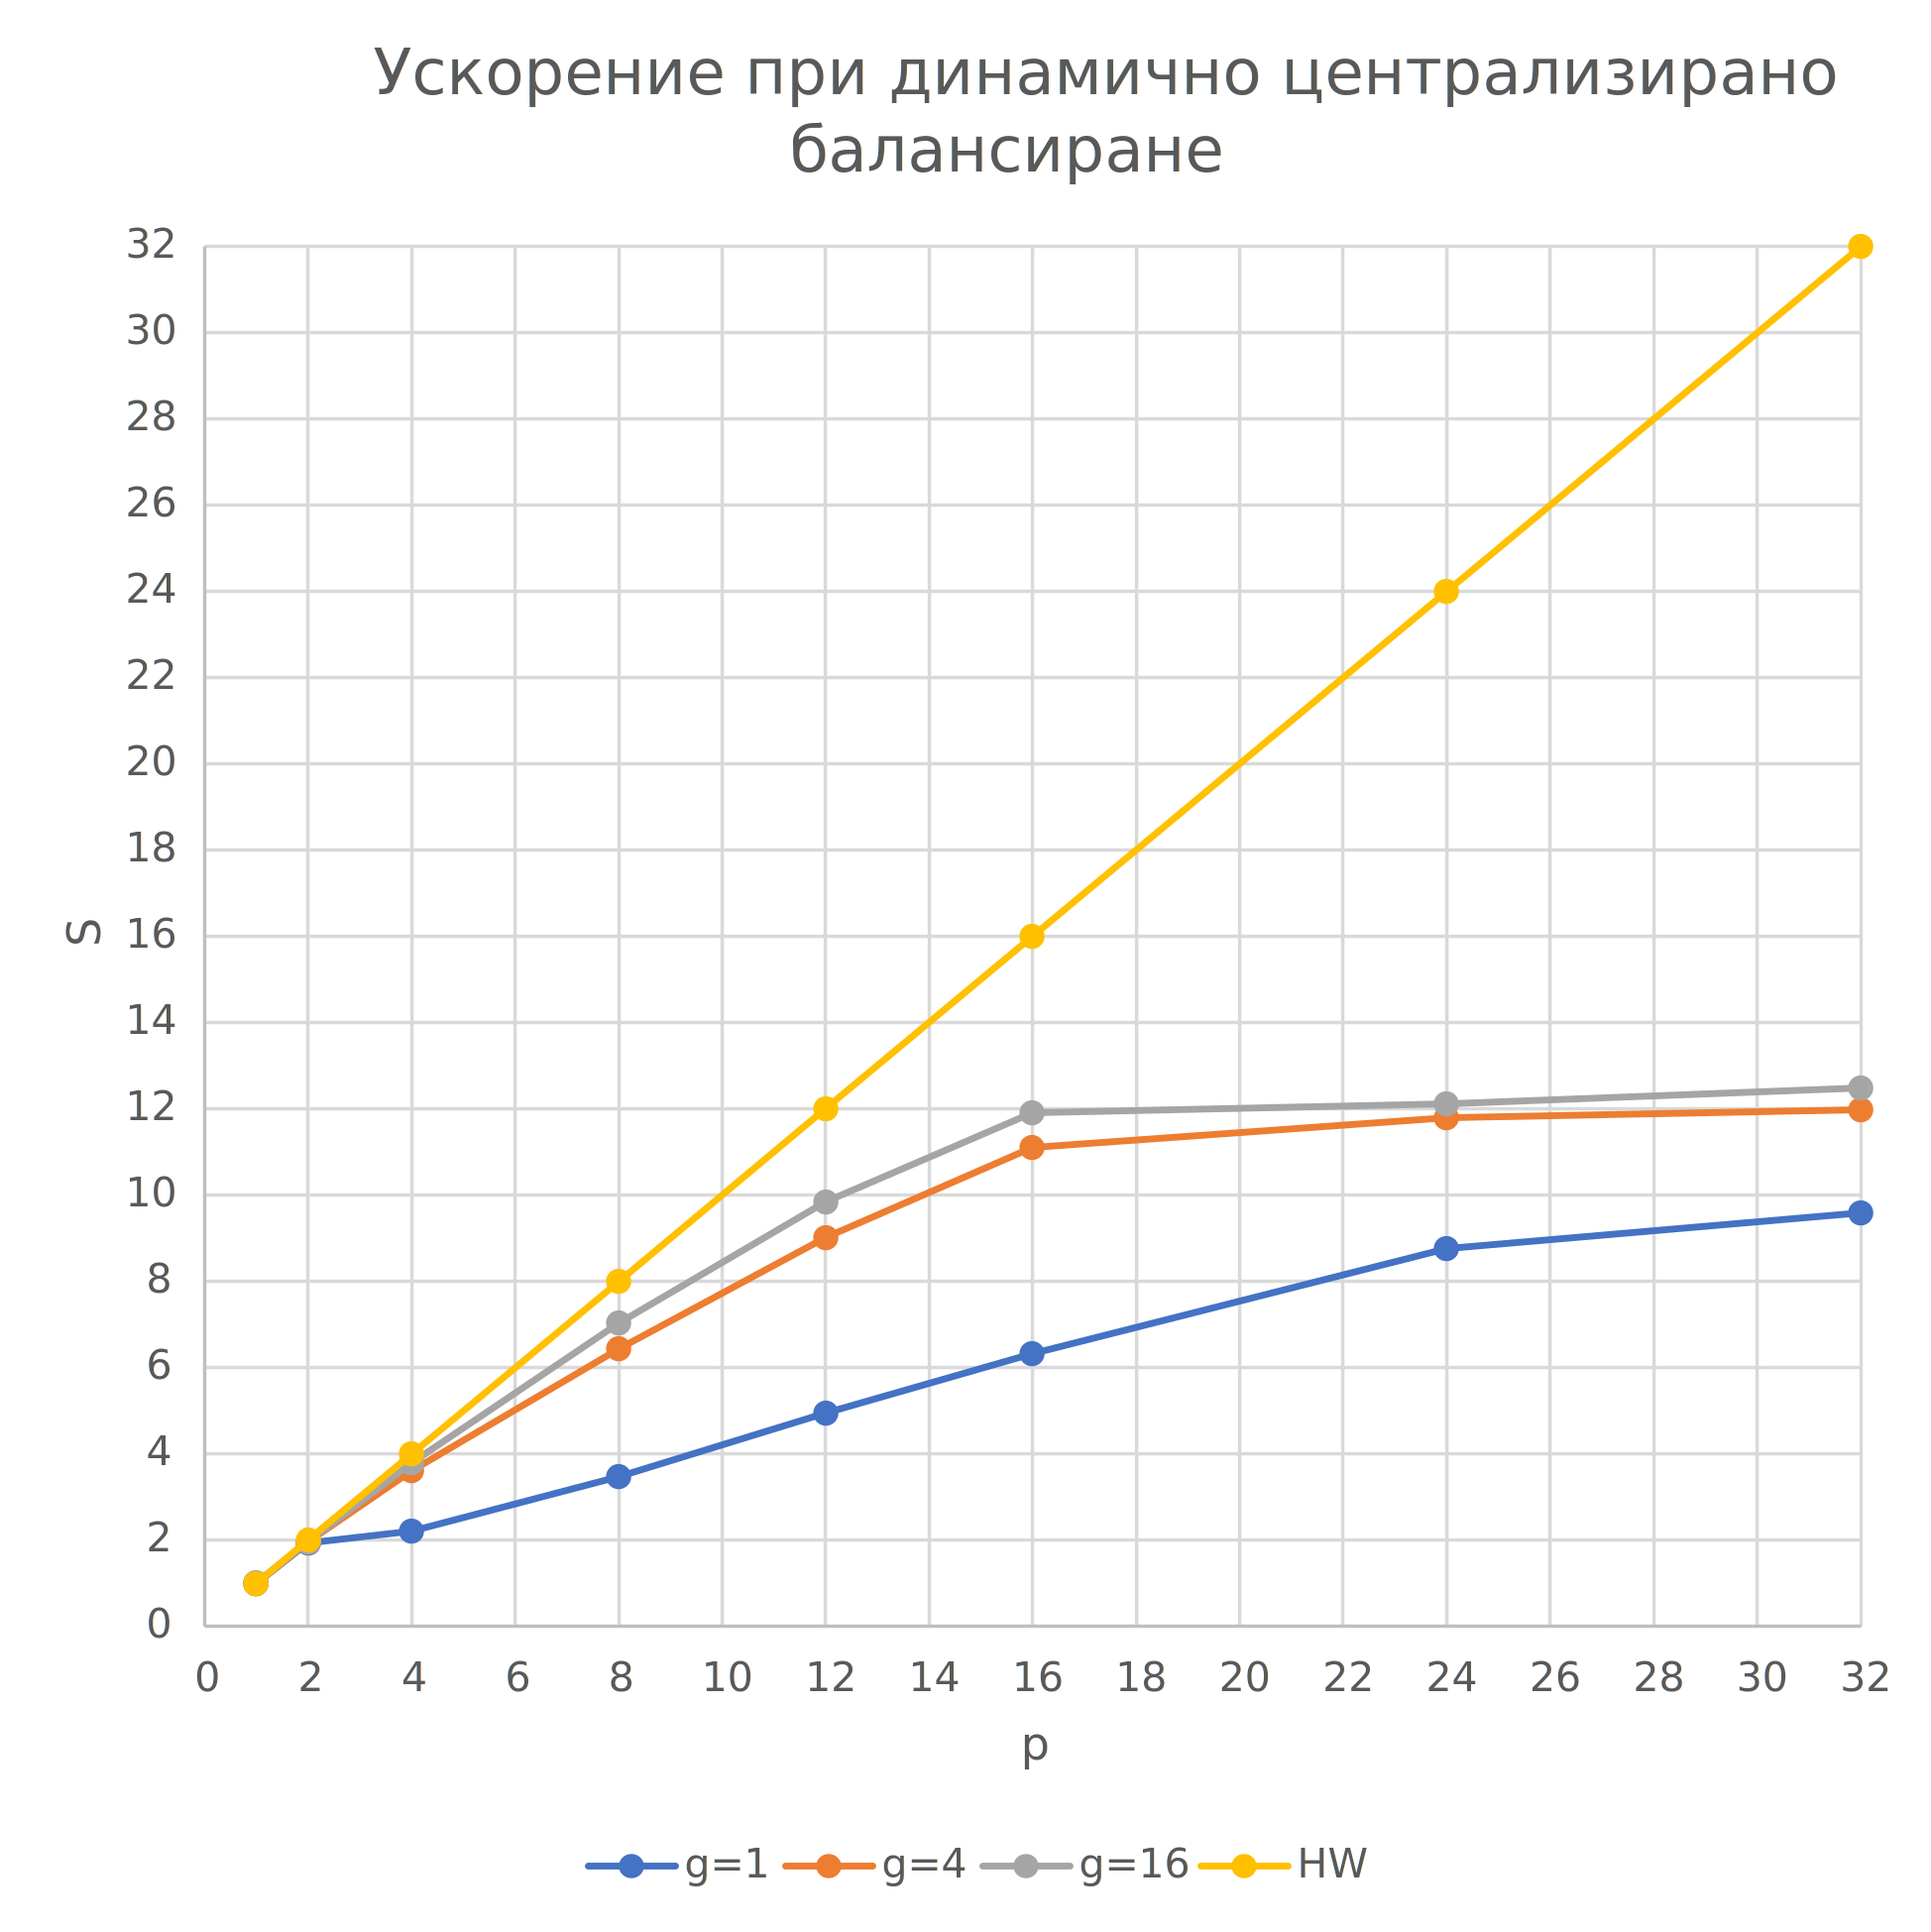
\includegraphics[width=0.9\linewidth]{images/DynamicMandelSpeedup.png}
    \caption{Ускорение при динамично балансиране}
    \label{fig:dynamic-speedup}
\end{figure}
\begin{figure}[H]
    \centering
    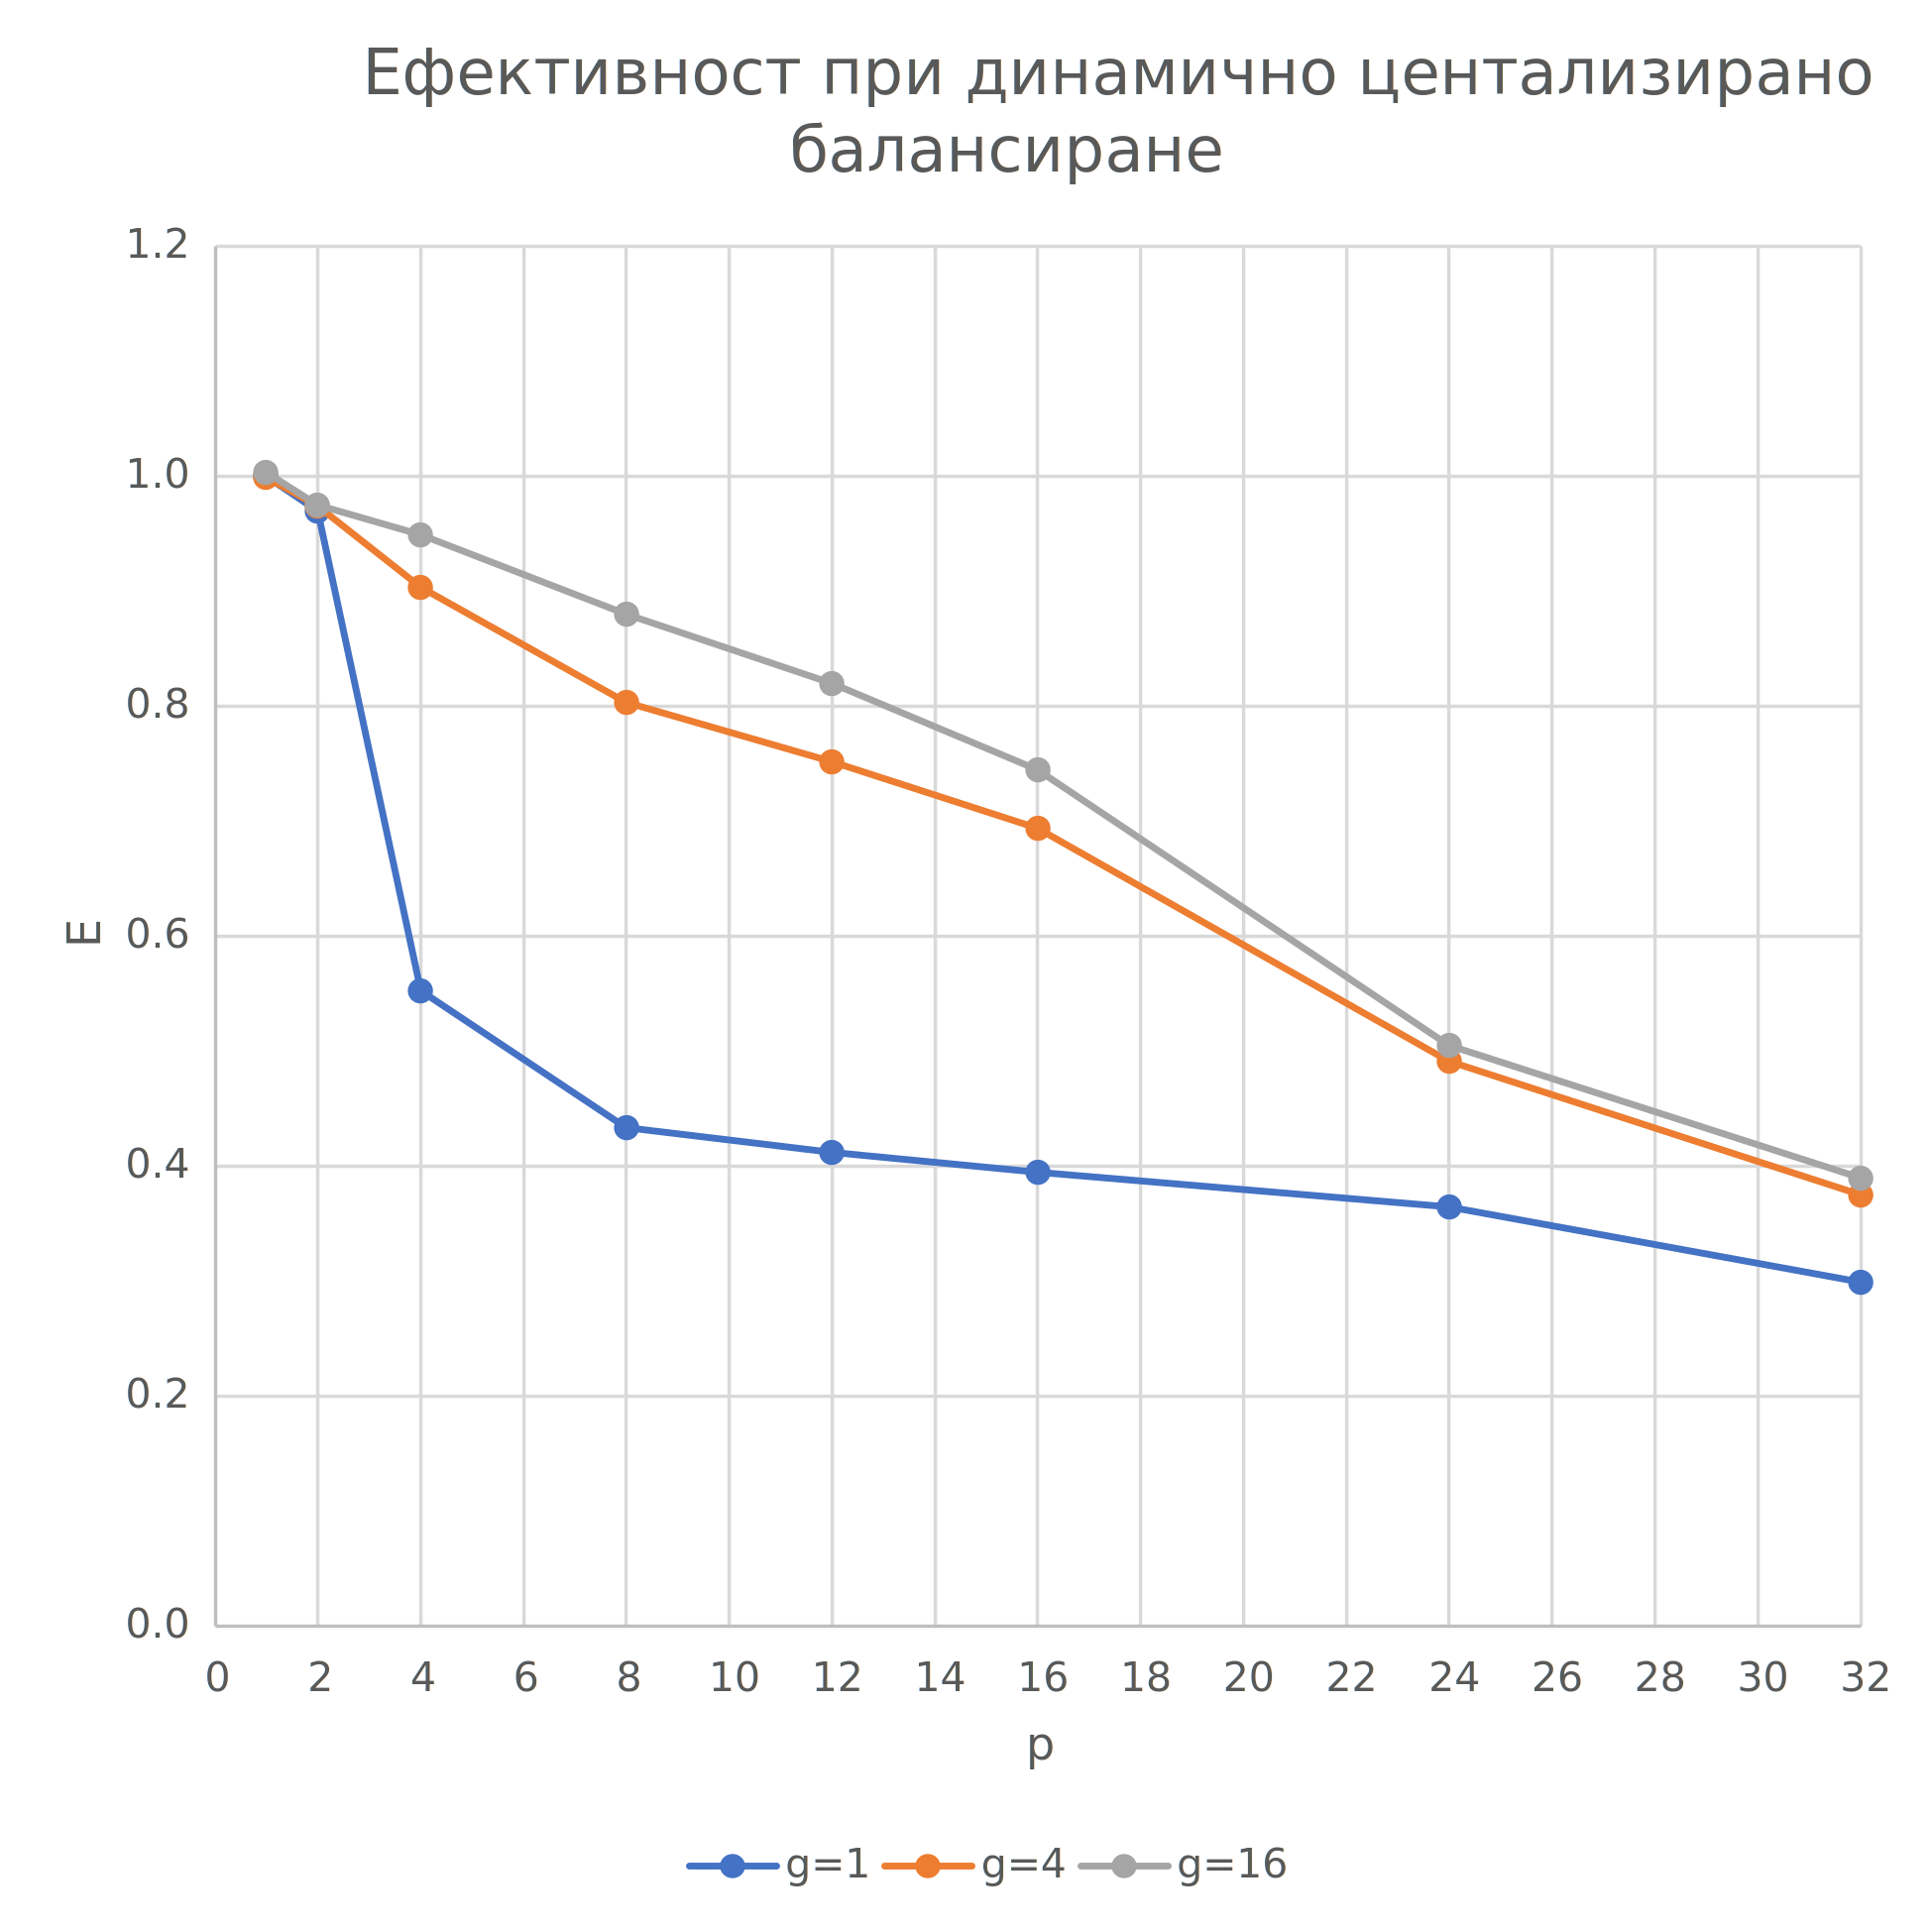
\includegraphics[width=0.9\linewidth]{images/DynamicMandelEffectiveness.png}
    \caption{Ефективност при динамично балансиране}
    \label{fig:dynamic-effectiveness}
\end{figure}

\begin{figure}[H]
    \centering
    \includegraphics[width=0.9\linewidth]{images/MandelComparisson.png}
    \caption{Сравнение на постигнатото ускорение при статично циклично и динамично централизирано балансиране}
    \label{fig:mandeltest-comparison}
\end{figure}
Резултатите от тестването на имплементацията с динамично централизирано балансиране са близки до тези от имплементацията със статичното циклично - максималното ускорение отново се постига при $p=32, g=16$. 
Отново липсват немотонни аномалии. В този случай се проявява хиперлинейна аномалия за $p=1, g=16$. 
Ако сравним постигнатото ускорение при статично циклично и динамично централизирано балансиране, в почти всички случаи статичното циклично балансиране превъзхожда по постигнато ускорение динамичното централизирано балансиране. Резултатът е очакван, с оглед на склонността на динамичното балансиране да поражда комуникационен свръхтовар. 
% \bibliographystyle{plain} 
% \bibliography{MyReferencesFile} % References are stored in MyReferencesFile.bib
\cleardoublepage
\section{Източници}
\paragraph{}[1] \textbf{Leduc, Ryan}, McMaster University, Toronto, Canada. 2004. \emph{Embarrassingly Parallel Computations.}. http://www.cas.mcmaster.ca/~leduc/slides4f03/slides6.pdf.
\paragraph{}[2] \textbf{Gamage, Bhanuka M., Vishnu M. Baskaran}, Monash University Malaysia. 1.07.2020. \emph{Efficient Generation of Mandelbrot Set using Message Passing Interface.} Arxiv. \\https://arxiv.org/pdf/2007.00745.pdf.
\paragraph{}[3] \textbf{Tracolli, Mirco, Antonio Lagana, Leonardo Pacifici}, University of Perugia. 21.04.2016. \emph{Parallel generation of a Mandelbrot set.} UniPG. \\http://services.chm.unipg.it/ojs/index.php/virtlcomm/article/view/112/108.
\paragraph{}[4] \textbf{Gomez, Erstesto S.}, Universidad de las Ciencias Informáticas, Cuba. 30.09.2020. \emph{MPI vs OpenMP: A case study on parallel generation of Mandelbrot set.} Redalyc. \\https://www.redalyc.org/journal/6738/673870835002/html/.
\cleardoublepage
% \phantomsection
\addcontentsline{toc}{section}{\listfigurename}
\listoffigures
% \phantomsection
\addcontentsline{toc}{section}{\listtablename}
\listoftables
\addcontentsline{toc}{section}{Списък на кода}
\lstlistoflistings{}
\end{document}